\chapter{
Introduction to Spatial Capture-Recapture
}
\markboth{Introduction}{}
\label{chapt.intro}


\vspace{.3in}

Information about abundance or density of populations, and their vital
rates, is fundamental to applied ecology and conservation biology.  To
that end, a huge variety of statistical methods have been devised, and
among these, the most well-developed are collectively known as
capture-recapture (or capture-mark-recapture) methods. For example,
the volumes by \citet{seber:1982}, \citet{borchers_etal:2002},
\citet{williams_etal:2002}, and \citet{amstrup_etal:2005} are largely
synthetic treatments of such methods, and contributions on modeling
and estimation using capture-recapture are plentiful in the
peer-reviewed ecology literature.  Capture-recapture techniques make
use of individual encounter history data, by which we mean sequences
of 0's and 1's denoting if an individual was encountered at a
particular trap during a certain time period. For example, the
encounter history ``010'' indicates that this individual was
encountered only during the second of three trapping occasions. As we
will see, these data contain
information about encounter probability, abundance, and other
parameters of interest in the study of population dynamics.

A diverse and growing number of methods exist for obtaining encounter
history data. Such methods are, naturally, taxa-specific. They include
classical ``traps'' which capture and retain animals until visited by
a biologist who removes the individual, marks it, or otherwise molests
it in some scientific fashion.  Small-mammal traps and mist nets for
birds are standard examples. Traps that physically capture and
restrain individuals are common, but capture-recapture methods no
longer require ``capture'' or even physical marking of individuals.
Recent technological advances have produced a
large number of passive detection devices that produce individual
encounter history data. These include camera traps
\citep{karanth_nichols:1998, oconnell_etal:2010}, acoustic recording
devices \citep{dawson_efford:2009}, and methods that obtain DNA
samples such as hair snares for bears \citep{gardner_etal:2010jwm}, scent
posts for many carnivores \citep{kery_etal:2010}, and related methods which allow DNA
to be extracted from scat, urine or animal tissue in order to identify
individuals.  This book is concerned with how such data can be used to
carry out inference about animal abundance or density, and other
demographic parameters such as survival, recruitment, and movement
using new classes of capture-recapture models which utilize auxiliary
spatial information related to the encounter process.  We refer to
such methods as spatial capture-recapture (SCR) models\footnote{In
the literature the term spatially explicit capture-recapture (SECR) is
also used}.

As the name implies, the primary feature of SCR models that
distinguishes them from traditional CR methods is that they make use
of the spatial information inherent to capture-recapture studies. That
is, the encounter histories are associated with spatial coordinates,
and these coordinates are informative about home range
characteristics, movement and space usage.
As we will see, this allows us to overcome three critical
deficiencies of non-spatial methods, namely,
traditional CR methods cannot be used to formally estimate density,
include of trap-level covariates of density or capture probability, or
account for heterogeneity in encounter probability that
results from the spatial organization of animals and traps.
Thus, spatial modeling is not just
a fun academic exercise; it provides a solution to basic problems in
the study of animal populations that have been acknowledged for more
than 70 years \citep{dice:1938}.

Before discussing how SCR resolves
these issues, we provide a brief overview of standard methods for
collecting spatial capture-recapture data, and we discuss the origins
of spatial capture-recapture methods.



\section{Lions and Tigers and Bears, oh my:  Genesis of
Spatial capture-recapture data}

A diverse number of methods and devices exist for producing individual
encounter history data with auxiliary spatial information about
individual locations. Historically, physical ``traps'' have been widely
used to sample animal populations. These include live traps, leg-hold
traps, mist nets, pitfall traps and many other types of
devices. Although these are still widely used, huge advances have been
made in developing new methodologies for obtaining encounter history
data non-invasively. We briefly review some of these here, which we
will consider more explicitly in later chapters of this book.

\subsection{Camera trapping}

Considerable recent work has gone into the development of
camera-trapping methodologies. For a historical overview of this
method see \citet{kays_etal:2008, kucera_barrett:2011}.  Several
recent synthetic works have been published including
\citet{nichols_karanth:2002}, and an edited volume by
\citet{oconnell_etal:2010} devoted solely to camera trapping concepts
and methods. As a method for estimating abundance some of the earliest
work that relates to the use of camera trapping data in
capture-recapture models originates from Karanth and colleagues
\citep{karanth:1995, karanth_nichols:1998, karanth_nichols:2000}. In
studies that use camera trapping, cameras are situated along trails or
at baited stations and individual animals are photographed and
subsequently identified either manually by a person sitting behind a
computer,  or sometimes now using computational
methods. Camera trapping methods are widely used for species that have
unique stripe or spotting patterns such as tigers \citep{karanth:1995,
  karanth_nichols:1998}, ocelots
\citep{trolle_kery:2003,trolle_kery:2005}, leopards
\citep{balme_etal:2010}, and many other cat species.
% Scientific names
Camera traps are
also used for other species such as wolverines
\citep{magoun_etal:2011}, and even species that are less easy to
identify uniquely such as mountain lions and coyotes
(e.g. \citet{kelly_etal:2008}.  We note that even for species that are
not readily identified by pelage patterns, it is possibly to use
camera traps in conjunction with spatial capture-recapture models to
estimate density (see Chapter~\ref{chapt.scr-unmarked}).
%, if an initial sample of individuals can be collared
%or tagged in some way so that subsequent encounter by camera-traps can
%yield individual information. In this way, the probability of
%encounter can be estimated from the camera traps based on the
%pre-marked individuals, and this is applied to the frequencies of
%unmarked individuals to estimate density.


\begin{figure}
\begin{center}
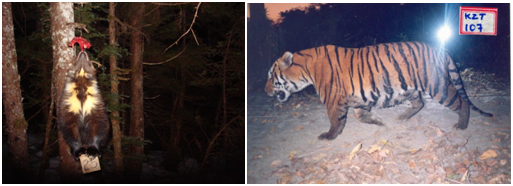
\includegraphics[width=5in]{Ch1/figs/wolverinetiger}
\end{center}
\caption{Wolverine in camera trap from A. Magoun (left). Picture of Tiger in
  camera trap from U. Karanth (right)}
\label{fig.wolverinetiger}
\end{figure}

\subsection{DNA Sampling}

Recent technological advances in the extraction and analysis of
genetic information have made a huge positive impact on the study of
animal populations. DNA obtained from hair, blood or scat is now
routinely used to obtain individual identity and encounter history
information about individuals \citep{taberlet_bouvent:1992,
  woods_etal:1999, mills_etal:2000, schwartz_monfort:2008}.  A common
method is based on the use of ``hair snares'' (Fig. \ref{fig.bearcat})
which are widely used to study bear populations
\citep{woods_etal:1999, gardner_etal:2010, garshelis_etal:2006,
  kendall_etal:2009}.  A sample of hair is obtained as individuals
pass under or around barbed-wire (or other physical mechanism) to take
bait. Hair snares have also been used to sample felid populations
\citep{garciaalaniz_etal:2010} and other species. DNA information can
also be extracted from urine and as a result DNA can be used to study
feline populations which are attracted to scent-sticks and deposit
urine which is subsequently analyzed in the lab
\citep{valiere_taberlet:2000, kery_etal:2010}.


\begin{figure}
\begin{center}
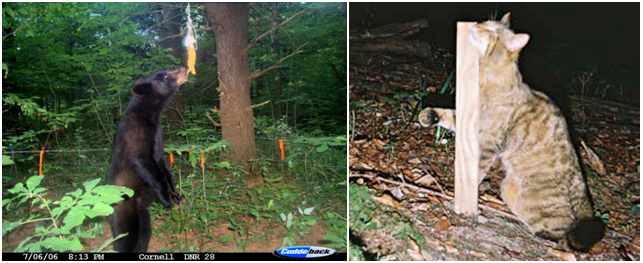
\includegraphics[width=5in]{Ch1/figs/bearcat}
\end{center}
\caption{Picture of hair snare. Bear (left). European wildcat
  (right). Pictures from??}
\label{fig.bearcat}
\end{figure}

\begin{figure}
\begin{center}
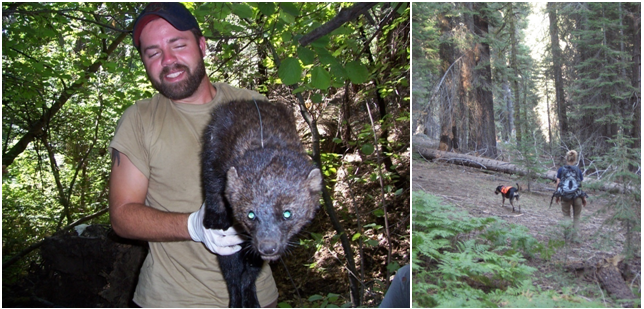
\includegraphics[width=5in]{Ch1/figs/beardog}
\end{center}
\caption{Guy holding fisher (left). Scat dog team working the ground
  (right). Pictures from Craig Thompson.}
\label{fig.fisherscatdog}
\end{figure}


\subsection{Acoustic surveys}

Many studies of birds, bats, and whales now collect data using
devices that record vocalizations.

\subsection{Search-Encounter Methods}

There are other methods which don't fall into a nice clean taxonomy of
``devices''. Spatial encounter histories\footnote{defined? probably
  not! need to do that} are commomnly obtained by conducting manual
searches of geographic sample units such as quadrats, transects or
road or trail networks.
For example,
DNA-based encounter histories can be obtained from scat
samples located along roads or trails or by specially trained dogs
\citep{mackay_etal:2008} searching space
(Fig. \ref{fig.fisherscatdog}). This method has been used in studies
of martens, fishers \citep{thompson_etal:inpress}, lynx, coyotes,
birds \citet{kery_etal:2010}, and many other species. We might search
space on foot and pick up individuals and physically mark them
somehow. This is pretty common in surveys that involve reptiles and
amphibians, e.g., we might walk transects through a forest and pick-up
box turtles \citep{hall_etal:1999} or search space for lizards
\citep{royle_young:2008} and also surveys designed to obtain animal
scat. These methods don't seem like normal capture-recapture in the
sense that the encounter of individuals is not associated with
specific trap location, but SCR models are equally relevant for
analysis of such data (see Chapter XY and XXX).


\section{ Historical Context: A Brief Synopsis of the Literature}

Spatial capture-recapture is a relatively new methodological
development, at least with regard to formal estimation and
inference. However, the basic problems that motivate the need for
formal spatially-explicit models have been recognized for decades and
quite a large number of ideas have been proposed to deal with these
problems. We review some of these ideas here.


\subsection{Buffering}

 The standard approach even now is to estimate $N$ using
conventional closed population models \citep{otis_etal:1978} and then
try to associate with this estimate some specific sampled area, say $A$,
the area which is contributing individuals to the population for which
$N$ is being estimated. The strategy is to define $A$ by placing a buffer
of say $W$ around the trap array or some polygon which encloses the trap
array. The historical context is succintly put by \citep{obrien:2011}
from which we draw this description:

\begin{quote}
  ``At its most simplistic, $A$ may be described by a concave polygon
  defined by connecting the outermost trap locations ($A_{tp}$; Mohr
  1947). This assumes that animals do not move from outside the
  bounded area to inside the area or vice versa. Unless the study is
  conducted on a small island or a physical barrier is erected in the
  study area to limit movement of animals, this assumption is unlikely
  to be true. More often, a boundary area of width $W$ ($A_{w}$) is added to
  the area defined by the polygon $A_{tp}$ to reflect the area beyond the
  limit of the traps that potentially is contributing animals to the
  abundance estimate (Otis et al. 1978). The sampled area, also known
  as the effective area, is then $A(W) = A_{tp} + A_{w}$. Calculation of the
  buffer strip width ($W$) is critical to the estimation of density and
  is problematic because there is no agreed upon method of estimating
  $W$. Solutions to this problem all involve ad hoc methods that date
  back to early attempts to estimate abundance and home ranges based
  on trapping grids
  \citep[see][]{hayne:1949}. \citet{dice:1938} first drew attention
  to this problem in small mammal studies and recommended using
  one-half the diameter of an average home range. Other solutions have
  included use of inter-trap distances (Blair 1940; Burt 1943), mean
  movements among traps, maximum movements among traps (Holdenried
  1940, Hayne 1949), nested grids \citep{otis_etal:1978}, and assessment
  lines (Smith et al. 1971).''
\end{quote}

The idea of using 1/2 mean maximum distance moved
\citep{wilson_anderson:1985a} seems to be the standard approach even
today, presumably justified by Dice''s suggestion to use 1/2 the home
range diameter. Alternatively, some studies have used the full
MMDM\footnote{Do they really say that?}
(e.g. \citet{parmenter_etal:2003}). And, sometimes home range size is
estimated by telemetry \citep{karanth:1995}\footnote{Is this correct
  cite for this?}. This is usually combined
with an AIC-based selection from among the closed-population models in
\citet{otis_etal:1978} which most often suggests heterogeneity (Model
Mh).  Almost all of these early methods were motivated by studies of
small mammals using classical ``trapping grids'' but, more recently,
their popularity has increased with the advent of new technologies and
especially related to non-invasive sampling methods such as camera
trapping. In particular, the series of papers by Karanth and Nichols
\citep{karanth:1995, karanth_nichols:1998, karanth_nichols:2002}
has led to fairly widespread adoption of these ideas.

Some of the heuristic ideas based on buffer strips do have some
technical justification in the sense of estimating parameters of an
underlying movement model from observed movements. For example, if we
let $x$ be a random variable indicating movement outcomes of an
individual about its  home range center, and suppose that $x$ has pdf
$g(x)$ then we can understand properties of MMDM by studying the
properties of the sample order statistics, as the maximum distance
moved is the sample range based on a sample of observations of
individual locations.

XXXX complete this thought XXXX

Problem is that N does not scale with A

XXXX                       XXXX

%As an illustration, imagine a 1-dimensional
%system where individuals have a home range that amounts to a line
%segment. Then suppose that individual movements are $\mbox{uniform}(0,A)$. It
%can be shown that the sampling distribution of the sample range, R,
%scaled by $A$, say $R/A$ has a beta distribution, $\mbox{beta}(n-1,2)$
%\citep[][p. 235]{casella_berger:2002}
%and thus the diameter of the home range, i.e. $A$, is
%estimated (biasedly) by$ R/( (n-1)/(n+1) )$. For large $n$ we could then
%say that the sample range, i.e., ''maximum distance moved'' seems like a good estimator of home range diameter and, therefore, $R/2$ is an estimator of home-range radius.

%There are a number of technical issues that arise in attempting to use
%such heuristics to justify the application in practice. For one, the
%moments of the sample order statistics are strongly affected by sample
%size, which is typically quite small (per individual encountered) and
%thus, in general, are biased and estimated with variable precision
%depending on sample size. For example, the expected value of MMDM is
%$k(n)*A$ , i.e., the true home range diameter is related to observed
%MMDM by some function of sample size, $k(n)$, that increases to 1. In
%the case where the underlying movement model is uniform, $k(n) =
%(n-1)/(n+1)$ (from above) which motivates a formula for ``adjusting''
%observed MMDM for small sample size. We suspect that many such
%formulae are obtainable depending on the assumed movement distribution
%\citep[e.g., formula 6.16 in][]{obrien:2011}. We might also think about taking
%the {\it maximum} (over individuals) of the maximum distance moved
%because under the specific model considered here (iid uniform) then
%all individuals have the same home range radius. This increases our
%sample size ($n$) and thus the observed sample range should be more
%accurate.


%%Another issue of somewhat more importance (and less easy to
%rectify) is that the {\it observation} of movement outcomes is biased
%by the locations of traps. We cannot observe movements ``off the
%trapping grid'' (or between traps) and thus our observed movements
%will generally be smaller than expected under any particular model
%(the uniform in this case). Moreover, the trap spacing also induces a
%discreteness to the movements that causes a further level of
%approximation based on hypothetical movement
%distributions. Nevertheless, formal analysis of `` buffering''
%strategies based on sample order statistics under specific models for
%movement does at least provide some heuristic support for specific
%choices.  The interested reader should ponder the distribution of the
%sample minimum, maximum and range under other distributions such as a
%normal (and bivariate normal), exponential distribution and perhaps
%others. In addition, contemplate the effect of censoring of movements
%to some arbitrary limit ($B<A$) to mimic bias in observed movement
%outcomes due to a finite trap grid.

\subsection{Trapping webs}

The use of buffer strips is conventional and widespread due to the
heuristic appeal of that idea and its easy implementation, but other
conceptual approaches exist to address specific problems motivated by
the spatial context of capture-recapture data. D.R. Anderson came up
with the idea of the ``trapping web'' \citep{anderson_etal:1983} which
does not seem to have been widely adopted in practice.
% although there
%is a clear mathematical formalization to the trapping web design
%\citep{link_barker:1994}.
One reason for this is
the design is somewhat restrictive in the sense that it requires
a large number of traps be organized in close proximity to one
another, and it assumes that capture is certain at the web center.

\subsection{Temporary Emigration}

Another intuitively appealing idea is that by \citet{white_shenk:2000}
who discuss ``correcting bias of grid trapping estimates'' by
recognizing that the basic problem is like random temporary emigration
\citep{kendall_etal:1997} where individuals flip a coin with
probability $\phi$ to determine if they are ``available'' to be
sampled or not.  White and Shenk's idea was to estimate $\phi$ from
radio telemetry, as the proportion of time an individual spends in the
study area. They obtain the estimated super-population size by using
standard closed population models and then obtain density by $\hat{D}
= \hat{N}\hat{\phi}/A$ where $A$ is the nominal area of the trapping
array (e.g., minimum convex hull).  A problem with this approach is
that individuals that were radio collared represent a biased sample
i.e., you fundamentally have to sample individuals randomly from the
population {\it in proportion to their exposure to sampling} and that
seems practically impossible to accomplish\footnote{this seems to
  shoot down our Florida panther work}.  That said, the temporary
emigration analogy is a good heuristic for understanding SCR models
and has a precise technical relevance to certain models.

Another very interesting idea is that of using some summary of
``average location'' as an individual covariate in standard
capture-recapture models. \citet{boulanger_mclellan:2001} use
distance-to-edge (DTE) as a covariate in the Huggins-Alho type of
model. \citet{ivan:2012} uses this approach in conjunction with an
adjustment to the estimated $N$ obtained by estimating the proportion of
time individuals are ``on the area formally covered by the grid''
using radio telemetry.  We do not dwell too much on these different
variations but we do note that the use of DTE as an individual
covariate amounts to some kind of intermediate model between simple
closed population models and fully spatial capture-recapture models,
which we address directly in Chapter 3.
%We note that no adjustment
%based on telemetry information is necessary if one were simply to
%place a prior distribution on the individual covariate (which is not
%to say that telemetry data isn't useful, just that the same objective
%can be achieved without telemetry data).

While these procedures are all heuristically appealing, they are also
essentially ad hoc in the sense that the underlying model remains
unspecified or at least imprecisely characterized and so there is
little or no basis for modifying, extending or generalizing the
methods. These methods are distinctly {\it not} model-based procedures
even though they might well be heuristically appealing under specific
movement models. Despite this, there seems to be an enormous amount of
literature developing, evaluating and ``validating'' these literally
dozens of heuristic ideas that solve specific problems, as well as
various related tweeks and tunings of them and really it hasn't led to
any substantive breakthroughs that are sufficiently general or
theoretically rigorous.


\subsection{The modern age}

\citet{efford:2004} was the first to formalize an explicit model for
spatial capture-recapture problems in the context of trapping arrays.
He adopted a Poisson point process model to describe the distribution
of individuals and then what is essentially a distance sampling
formulation of the observation model which describes the probability
of detection as a function of individual location, regarded as a
latent variable governed by the point process model. While earlier
(and contemporary) methods of estimating density from trap arrays have
been ad hoc in the sense of lacking a formal description of the
spatial model, Efford achieved a formalization of the model,
describing explicit mechanisms governing the spatial distribution of
individuals and how they are encountered by traps, but
adopted a more or less ad hoc framework for inference under that
spatial model using a simulation based method known as inverse
prediction.

Recently, there has been a flurry of effort devoted to formalizing
inference under this model-based framework for the analysis of spatial
capture-recapture data. There are two distinct lines of work which
adopt the model-based formulation in terms of the underlying point
process but differ primarily by the manner in which inference is
achieved. One approach \citep{borchers_efford:2008} is a classical inference approach based on
likelihood, and the other \citep{royle_young:2008} adopts a
Bayesian framework for inference.

To motivate the origins and relevance of these approaches, we note
that, fundamentally, spatial capture-recapture models are related to
classical ``individual covariate'' models (colloquially referred to as
Huggins-Alho models) in capture-recapture \citep{huggins:1989,
  alho:1990}.  In particular, the individual covariate\footnote{have
  we mentioned what the individual covariate is, yet?} is observed in
these classical individual covariate models whereas it is not directly
observed in SCR models.  To accommodate that, a prior distribution for
the individual covariate is required. In essence then, SCR models are
similar to a fully model-based formulation of classical Huggins-Alho
models (see \citet{royle:2009}). Likelihood analysis
\citep{borchers_efford:2008} proceeds by removing the random effect
from the likelihood by integration whereas Bayesian analysis
\citep{royle_young:2008} proceeds by analyzing the conditional model
directly, usually by methods of Markov chain Monte Carlo (MCMC).


%A classical argument in favor of the HA model is
%that it ``doesn't require assumptions about the covariate'' but the
%assumption is explicit in capture-recapture models and thus it is
%natural to attack inference based on the ``joint likelihood''
%\citep{borchers_etal:2002}. This has proven necessary in certain other
%classes of individual covariate models in which natural models arise
%for the individual covariate, such as time-varying individual
%covariates \citep{bonner_schwarz:2006}, or covariates with measurement
%error (e.g., distance sampling; see
%\citet[][ch. 7]{royle_dorazio:2008}).
%The model-based formulation is easily adapted to standard
%individual covariate models as well \citep{royle:2008}. Throughout
%this book we rely heavily on Bayesian inference of the joint
%likelihood, using the formulation based on data-augmentation
%\citep{royle_etal:2007, royle_young:2008, royle:2009} though we also
%discuss the development of likelihood-based inference in chapter 5 and
%apply those methods in some cases.


\section{The Failure of Classical Capture-Recapture}

The basic story is that Classical ``non-spatial'' C-R methods are
distinctly non-spatial. They don't admit spatial indexing of sampling
(observation) or
of individuals (process). This leads immediately to 3 main deficiencies:
 (1) there is no coherent basis for estimating density
 (2) non-spatial models {\it induce} a form of heterogeneity that can
 only at best be approximate by classical models of latent heterogeneity
 (3) ordinary models do not accommodate trap-level covariates which
 exist in a preponderance of studies.

ANDY STOPPED HERE


We confront some of the issues that motivate the need for spatial
capture-recapture models by considering analysis of data from a study
design to estimate black bear abundance on the Fort Drum Military
Installation in upstate New York (see Ch. 3 for more details). The
specific data used here are encounter histories on 47 individuals
obtained from an array of 38 baited ``hair snares'' during June and
July 2006. The study area and locations of the 38 hair snares are
shown in Fig. \ref{fig.hairsnares}.  Barbed wire traps (see
Fig. \ref{fig.bearcat}) were baited and checked for hair samples each
week for eight weeks.  Analysis of these data appears in
\citet{gardner_etal:2010jwm} and we use the data in a number of analyses
in later chapters.

\begin{figure}
\begin{center}
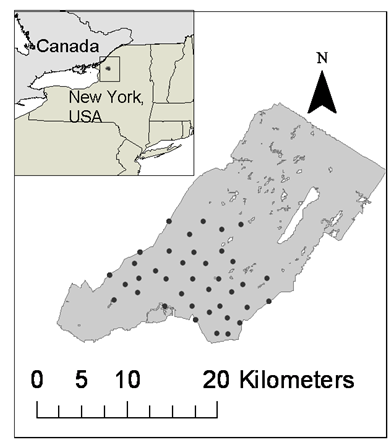
\includegraphics[height=3in]{Ch1/figs/hairsnares}
\end{center}
\caption{Locations of black bear hair snares on Fort Drum.}
\label{fig.hairsnares}
\end{figure}

We regarded this data set as a standard capture-recapture data set -
an encounter history matrix with 47 rows and 8 columns with entries
$y_{ik}$, where $y_{ik}=1$ if individual $i$ was captured in sample
$k$ and $y_{ik}=0$ otherwise. There is a standard closed population
model, colloquially referred to as ``Model M0'' (see Ch. 3), which
assumes that encounter probability $p$ is constant for all individuals
and sample periods.  We fitted Model M0 to the Fort Drum data using
traditional likelihood methods, yielding the maximum likelihood
estimate (MLE) of $\hat{N} = 49.19$ with an asymptotic standard error
(SE) of $1.9$.

The key issue in using closed population models with such data is how
on earth do we interpret this estimate of $N=49.19$ bears? Does it
represent the entire population of Fort Drum? Certainly not -- we merely sampled half of the Fort! So to get at the total bear population size of Fort Drum , we'd have to convert our $\hat{N}$ to an estimate of density and extrapolate. To get at density, then, should we
assert that $N$ applies to the southern half of Fort Drum below some
arbitrary line? Surely bears move on and off of Fort Drum without
regard to hypothetical boundaries. Without additional information
there is simply no way of converting this estimate of $N$ to density,
and hence it is really not meaningful biologically. To resolve this
problem, we will adopt the customary approach of converting $N$ to $D$
by buffering the convex hull around the trap array. The convex hull
has area $157.135$ $km^2$. We follow \citet{bales_etal:2005} in
buffering the convex hull of the trap array by the radius of the mean
female home range size\footnote{Did Bales et al. actually do this?}.
The mean female home range radius was
estimated \citep{wegan:2008} for our study region to be $2.19$
km\footnote{Is this number right out of Wegan's disseration?}, and
the area of the convex hull buffered by $2.19$ km is $277.01$
km$^2$. ({\bf R}
commands to compute the convex hull, buffer it, and compute the area
are given in the {\bf R} package \mbox{scrbook} which accompanies the
book).  Hence, the estimated density
here is approximately $0.178$ bears/km$^2$ for an estimated population
size obtained using Model $M_0$.  We could assert that the problem has
been solved, go home, and have a beer.  But then, on the other hand,
maybe we should question this estimated home range radius from
\citep{wegan:2008} -- after all, home ranges can change for many reasons. Instead, we may decide to rely on a buffer width based on
one-half MMDM estimated from the actual hair snare data as is more customary
\citep{dice:1938}. In that case the buffer width is $1.19$ km, and the
resulting estimated density is increased to $0.225$ bears/ha$^2$ about
27 \% larger.  But wait - some studies actually found the full MMDM
\citep{parmenter_etal:2003} to be a more appropriate measure of
movement (e.g \citet{soisalo_cavalcanti:2006}). So maybe we should use
the full MMDM
which is $2.37$ km, pretty close to the telemetry-based estimate
and therefore providing a similar estimate of density ($0.171$
bears/ha$^2$). So in trying to decide how to buffer our trap array we
have already generated 3 density estimates. The crux of the matter is
obvious: Although it is intuitive that $N$ should scale with area --
the number of bears should go up as area increases and go down as area
decreases -- in this ad hoc approach of accounting for animal movement
$N$ remains the same, no matter what area we decide we sampled. The
number of bears and the area they live in are not formally tied
together within the model, because estimating $N$ and estimating the
area $N$ refers to are two completely independent analytical steps.

Unfortunately, our problems don't end here. In thinking about the use of model M0, we might naturally question
some of the basic assumptions that go into that model. The obvious one
to question is that which declares that $p$ is constant. One obvious
source of variation in $p$ is variation {\it among individuals}. We
expect that individuals may have more or less exposure to trapping due
to their location relative to traps.
%Maybe we could add a table of how many traps each bear was caught in
% #traps: 1   2  3  4  5  6  7  8 10
% #bears: 19 15  5  2  2  1  1  1  1

This has led many to consider
capture-recapture models that allow for individual heterogeneity in
$p$. Such models have the colloquial name of ``Model Mh.''
We fitted this model (see ch. 3 for details) to the Fort Drum data
using each of the 3 buffer widths previously described (telemetry, 1/2
MMDM and MMDM), producing the estimates reported in Table
\ref{tab.fdests}. While we can tell by the models' AIC that Mh is
clearly favored by more than 30 units, we might still not be entirely
happy with our results. Clearly there is information in our data that
could tell us something about the exposure of individual bears to the
trap array -- where they were captured, and how many times -- but
since space has no representation in our model, we can't make use of
this information. Model Mh thus merely accounts for what we observe in
our data (some bears were more frequently captured than others) rather
than explicitly accounting for the processes that generated the data.

So what are we left with?  Our density estimates span  a range
from $0.17$ to $0.43$ bears/km$^2$ depending on which estimator of $N$ we use and
what buffer strip we apply. Should we feel strongly about one or the other?
AIC favors model Mh, but did it adequately account for the differences in exposure of individuals to the trap array? If so, which buffer should we
prefer? \footnote{Give AIC of models in table. Andy to finish. }
%Moreover, we could find more variations of
%model Mh to choose among, but see \citep{link:2003}.
And if we choose one type of buffer, how do we compare our density estimates to those from other studies that may opt for a different kind of buffer?
Clearly, there is no compelling solution to deriving density from our
estimate of $N$, and we are left not much wiser about bear density at
Fort Drum than we were before we conducted this analysis.

%%%% We could just finish this part off with a paragraph about these additional open questions - the whipped cream of problems on the capture-recapture sundae - including the trap-level covariates; or we could come up with some trap-level covariate example for the bears (different baits used, blabla).
Some of the open questions at this point:
How do we characterize uncertainty of the buffer ``estimate''?  And,
in what sense is the
buffer even an estimate of something? What is it an estimate of?
The summary here should be that there's not a compelling solution to be derived from
this ``estimate $N$ conjure up a buffer'' approach.
{\bf The main point that N doesn't scale with A is not made
  clearly here.}

\begin{table}[ht]
\centering
\caption{Table on estimates of D for the Fort Drum data
using M0 and Mh and different buffers.}
\begin{tabular}{ll|cc}
\hline
model & buffer &  $\hat{D}$ & SE \\ \hline
M0   & telemetry &  0.178 & 0.178 \\
M0    & MMDM     &  0.171 & 0.171\\
M0   & 1/2 MMDM  &  0.225 & 0.225\\
Mh(ln) & telemetry &0.341 & 0.144\\
Mh(ln) & MMDM    &  0.327 & 0.138\\
Mh(ln) & 1/2 MMDM & 0.432 & 0.183\\
\end{tabular}
\label{tab.fdests}
\end{table}



\section{Extension of Closed Population Models}

The deficiency with classical closed population models is that they
have no spatial context. $N$ is just an integer parameter that applies
equally well to some population in a computer, estimating the number
of unique words in a book, or a bucket full of goldfish.  The question
of {\it where} the $N$ items belong is central both to interpretation
of data and estimates from all capture-recapture studies and, in fact,
to the construction of spatial capture-recapture models considered in
this book.  Surely it must matter whether the $N$ items exist as words
in a book, or goldfish in a bowl, or birds in a forest patch! That
classical closed population models have no spatial context leads to a
number of conceptual and methodological problems or limitations as we
have discussed and even encountered in our analyses so far.

Thus, the essential problem is that classical closed population models
are too simple - they ignore the spatial attribution of traps and
encounter events, movement and variability in exposure of individuals
to trap proximity, and they do not yield estimates of {\it density}.
These are not problems per se but rather just features
of this simple class of models, and they
should be addressed formally by the development of
more general models.  Spatial capture-recapture models are
statistical and mathematical models that extend non-spatial
``ordinary'' capture-recapture models to accommodate the spatial
structure inherent in sampling animal populations - i.e., trap
locations, individual locations, and individual use of space.

The solution to the various issues that arise in the application of
ordinary capture-recapture models is to extend the closed population
model so that $N$ becomes spatially explicit.  A natural way is to
define a point process \citep{efford:2004} that describes how
individuals are organized in space and that, when points are
aggregated over space, the value $N$ is derived in a meaningful way.
Thus, in this book, we adopt the view that the locations of the $N$
individuals in the population are a {\it realization of a spatial
  point process}.







\subsection{Abundance as the Aggregation of a Point Process}

Spatial point process models represent a major methodological theme in
spatial statistics \citep[][ch. xyz]{cressie:1992} and they are
widely applied as models for many ecological phenomena
\citep{stoyan_penttinen:2000,illian_etal:2008}. Point process models apply to
situations in which the random variable in question represents the
locations of events or objects: trees in a forest, weeds in a field,
bird nests, etc.  As such, it seems natural to describe the
organization of individuals in space using point process models.

One
of the key features of SCR models is that the point locations are
latent, or unobserved, and we only obtain imperfect information about
the point locations by observing individuals at trap or observation
locations.  Thus, the realized locations of individuals represent a
type of ``thinned'' point process, where the thinning mechanism is not
random but, rather, biased by the observation mechanism.  It is
natural to think about the observed point process as some kind of a
compound or aggregate point process with a set of ``parent'' nodes
being the locations of individual home ranges or their centroids,
and the observed locations as
``offspring'' - i.e., a Poisson cluster process (PCP). In that
context, density estimation in SCR models is analogous to estimating the number of
parents in the PCP \citep{chandler_royle:2012}.
% Other types of point
% process models for the realized locations have direct relevance to SCR
% models (See \citet{chandler_royle:2012}, discussed in chapter XYZ).

In the context of SCR models, we suppose there is a point on the
landscape that we'll think of as a home range center or, if this is
unappealing, we can think of it as the centroid of an individual's
activities during the time of sampling. In general, this point is
unknown for any individual but if we could track an individual over
time and take many observations then we could perhaps get a good idea
of where that point is.  We'll think of the collection of these points
as defining the spatial distribution of individuals in the
population. Most of the recent developments in modeling and inference
from spatial encounter history data, including most methods discussed
in this book, are predicated on the view that individuals are
organized in space according to a relatively simple point process
model. More specifically, we assume that the collection of individual
activity centers are ``$iid$'' random variables distributed uniformly
over some region. This is consistent with the assumption that the
activity centers represent the realization of a Poisson point process
or, if the total number of activity centers if fixed, then this is
usually referred to as a binomial point process.

%%I think we could shorten the home range paragraph; I like the definition
%%'the centroid of an individual's
%%% activities during the time of sampling'. I think the definition of
%% home range is something like the colleciton of points/sites/areas
%% an animal uses over the course of its lifetime so it's vague anyway
%% and what that definition means for the different forms of home
%%ranges - territory, migratory species etc - is pretty much left open.
We use the terms home range or activity center interchangeably. The
term ``home range center'' suggests that models are only relevant to
animals that exhibit such behavior of establishing home ranges or
territories and since not all species do that, perhaps the
construction of SCR models based on this idea is flawed. However,
 the notion of a home range center is just a conceptual
device and we don't view this concept as being strictly consistent
with classical notions of animal territories. Rather our view is
that a home range or territory is inherently dynamic, temporally, and thus it is a
transient quantity - where the animal lived during the period of
study.  Therefore, whether or not individuals of a species establish home ranges
is irrelevant because, once a precise time period is defined, this defines a distinct region of space
that an individual must have occupied. In other
words, the definition of ``home range center'' is predicated, in a
sense, on the specification of a time period over which individuals
are studied. A term that might be less offensive than ``home range
center'' is ``centroid of space usage (CSU)'' which should not
conflict directly with preconceived understandings and interpretations
of home range\footnote{Utilization distribution is the same thing
  I guess?}.


\subsection{The state-space}

If we let ${\bf s}_{i}; i=1,2,\ldots,N$ be the locations of individual
activity centers, then the question ``what are the possible values of
${\bf s}$?'' needs to be addressed because the individual ${\bf
  s}_{i}$ are {\it unknown}. As a technical matter, we will regard
them as random effects and in order to apply standard methods of
statistical inference we need to provide a distribution for these
random effects.  In the context of the point process model, the
possible values of the point locations referred to as the
``state-space'' of the point process and this is some region or set of
points which we will denote by ${\cal S}$.
${\cal S}$ is a region within which points are located - essentially a
prior distribution for ${\bf s}_{i}$ (or, equivalently, the random effects
distribution).
%%Don't think prior has come up yet; maybe not that important here?
In animal studies as a description of
where individuals that could be captured are located it encloses our
study area -- the region within which we might have located traps or
detection devices.  The state-space of the point process should
accommodate all individuals that could have been captured in the study
area.

In the practical application of SCR models, in most cases estimates of
density will be relatively insensitive to choice of state-space (see
Section XYZ)
%%% I also think the rest of this paragraph could be postponed to a later chapter
unless there are meaningful features to the state-space
which should be accommodated. For example, if the region within which
traps are located contains a coastline or a huge body of water then
clipping that out of the state-space will typically have a large
effect on density. This should be expected because, insofar as the
state-space serves as a prior distribution on the latent variables
${\bf s}_{i}$ then, {\it the state-space is very much a
  component of the model. } We discuss choosing the state-space in
Chapter 4.

When the underlying point process is well-defined, including a precise
definition of the state-space, this in turn induces a precise
definition of the parameter $N$ ``population size'' as the number of
individual activity centers located within the prescribed state-space.
A deficiency with some classical methods of ``adjustment'' is they
attempted to prescribe something like a state-space - a ``sampled
area'' - except absent any precise linkage of individuals with the
state-space. SCR models formalize the linkage between individuals and
space and, in doing so, provide an explicit definition of $N$
associated with
a well-defined spatial region, and hence
density. In a sense, the whole idea of SCR models is that by defining
this point process and its state-space ${\cal S}$, this gives context and
meaning to $N$ which can be estimated directly for that specific
state-space. Thus, it is fixing ${\cal S}$ that resolves the problem of
``unknown area'' that was addressed previously (Section XXXX).
%% I find the next two sentences a little confusing
But the
existence of an explicit state-space ${\cal S}$ is kind of beside the
point -- ${\cal S}$ is really not always terribly important
itself. Instead, as soon as you give the latent variables ${\bf s}$ a
place to live, and this is recognized explicitly in the model upon which inference is based,
 then you achieve spatial explicitness of the model.










%\begin{comment}

\subsection{Putting the pieces together}

Before we delve into the specifics of SCR, we want to provide a simple
conceptual overview and introduce some key notation. Our introduction
of SCR models follows our belief that models should closely reflect
the processes being studied. That is, it is always better to directly
model the ecological process of interest rather than just some index
that may or may not be related to the actual parameter in
question. For this reason, it is good to begin our discussion of SCR
models by simply describing what we think is happening in the real
world. We believe that few ecologists would argue with the following
three statements (the SCR postulates) that motivate the development of
SCR models:
{\flushleft \bf The SCR Postulates:}
\begin{itemize}
\item[1.] Animals are distributed in space and move about within some area (e.g., a home range).
\item[2.] Ecologists impose an array of traps or detection devices to sample the population.
\item[3.] Animals that live and move about in close proximity to traps are more likely to be encountered than those far from traps.
\end{itemize}
These statements are intuitive and hardly contentious, and they point
to two ecological processes (distribution and movement), and one
observation process (detection as a function of distance between a
trap and an animal's area of activity). SCR models assert statistical
descriptions for each of these three processes so that we can estimate
population density, model population dynamics, and study the processes
affecting distribution and movement.

As an example, let's assume that $N$ animals occur within an explicit
spatial region denoted by ${\cal S}$
(e.g., a polygon).  Each animal moves around some activity center
whose two-dimensional coordinates are denoted ${\bf s}_i;
i=1,2,...,N$. An animal's location at a specific point in time is
referenced by the coordinates ${\bf u}_{it}; t=1,2,...,T$. For
simplicity, let's assume that activity centers are uniformly
distributed in space, and movements are symmetric around these
activity centers. We now have a model of the ecological state process,
which we can write using the following notation
\[
{\bf s}_{i} \sim \mbox{Uniform}({\cal S})
\]
and
\[
{\bf u}_{it} \sim \mbox{Normal}({\bf s}_{i}, \sigma)
\]
To reiterate, these are statistical statements of two basic hypotheses
that (1) activity centers are uniformly distributed in two-dimensional
space, and (2) movements are normally distributed around the activity
centers. It is helpful to visualize this model by mapping the outcomes
of a single simulation. Below we provide simple R commands to do so.

{\small
\begin{verbatim}
set.seed(36372)       # so that results can be reproduced
N <- 10               # population size
                      # create trap coordinates:
x <- cbind(rep(seq(0.1,0.9,0.2), each=5), rep(seq(0.1,0.9,0.2), times=5))
                      # generate individual home range centroids
s <- cbind(runif(N), runif(N))
                      # create nice graphic:
plot(x, pch= "+", xlim=c(0,1), ylim=c(0,1), xlab="Easting", ylab="Northing")
points(s, pch=16, col="blue")
for(t in 1:5) {
  points(cbind(rnorm(N, s[,1], 0.05), rnorm(N, s[,2], 0.05)), col="green",pch=20)
}
\end{verbatim}
}

Fig. \ref{intro.fig.fig1} shows the results of executing these {\bf R} commands. The crosses
in the figure are trap locations, the blue circles are the locations
of each animal's activity center, and the green circles are animal
locations at 5 points in time.  The resulting plot not only
illustrates a simple state model for animal distribution and movement,
but it also hints at the potential influence of the distance between
animals and traps on the detection process. One would expect that the
traps in the northern part of the study area would capture more
animals than those in the south because fewer animals occur in the
south and movements are small. Clearly the encounter rate will also
depend upon the methods used to capture the animals, which we describe
in the next section.  Spatial capture-recapture models provide a
statistical formalization of these considerations.


\begin{figure}
\begin{center}
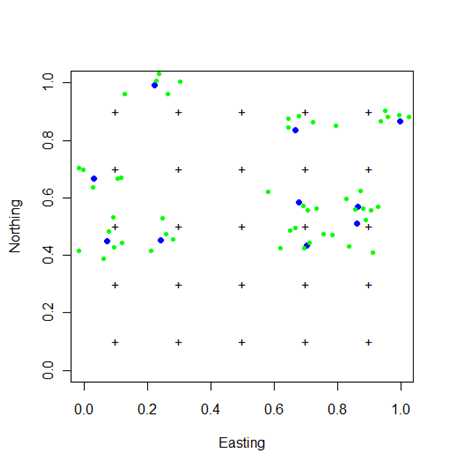
\includegraphics[height=3in]{Ch1/figs/northingeasting}
\end{center}
\caption{Population of $N$ individual home-range centers and locations
  during $K=5$ times. Also some trap locations.}
\label{intro.fig.fig1}
\end{figure}



%\end{comment}







\subsection{Other elements of SCR models}

Broadly speaking we differentiate
between two situations: Sampling based on fixed arrays or sampling
based on ``search encounter'' methods. The former includes things like
camera traps, hair snares, mist nets and conventional traps. Fixed
arrays limit the observation location to pre-defined points, where
traps are located. Using such methods the model is a little simpler
because the ``movement process'' of individuals is confounded with the
``observation process''.
The 2nd type of model -- search encounter models -- typically
will allow locations in continuous space, possibly only restricted by
polygon boundaries \citep{royle_young:2008}.
Search-encounter data
usually allow for the separate modeling and estimation of movement
model parameters from encounter model parameters but not always,
depending on whether replication of the sampling is done.  The
classical distance sampling model with no replication (i.e., $t=1$) is a basic model
which confounds the two processes.


Depending on the type of device being considered, certain restrictions
on the observable variable are induced which suggest specific
probability models for the observable random variable, suggesting
either binomial, Poisson or multinomial (and possibly other)
observation models.
One type of a
device is what we think of as the classical ``camera trap'' and which
\citet{efford:2011} refers to as a ``proximity detector''. We can take
pictures of or detect any number of individuals and an individual can
be caught in any number of traps, and an arbitrary number of
times. Iid Bernoulli model is convenient but if you think the
re-encounters are valuable then you can have a frequency model.  Bear
hair snares are slightly different because you cannot differentiate
re-encounters.
The standard observation model that applies for ``single-catch''
\citep{efford_etal:2004} traps posits that individuals are encountered
in at most one trap per sample occasion and traps only hold one
individual.  Unfortunately we're really screwed in the single-catch
situation.
A ``multi-catch'' is like a mist-net or other things - individual is
captured and restrained but traps hold > 1 individual. In this case,
the observation model is a multinomial. There are
many variations on all of these models and new models.

\begin{comment}
other things I have trouble working in here:

state-space: continuous, discrete, polygons???

observation locations: continuous, discrete, mapped to a polygon, or
something else?

auxiliary information e.g., from telemetry?

\subsubsection{5. modeling distance}

An important part of the observation model of every SCR model is the
manner in which {\it distance} between individuals and observation
locations (``sampler'') enters into the model.
This depends on whether the sampling is done at a point, along a line,
or uniformly over some polygon.

Observation location $x$ is a point.  We record individual location at
point $x$ or at some other location $u$. Distance is either $||x-s||$
or $||x-u||$.

Observation location is a ``line'':
(i) if we note point on line {\it and} $u$ then radial distance $||x - u||$
(ii) We don't observe point on line we might use ``closest distance''
(standar distance sampling)
(iii) we may or may not observe ${\bf u}$.
(iv) we might only record ${\bf u}$ but not the point on the line. In
that case we could use closest-distance or ``total hazard''.

More often, distance samplers approximate this with the closest linear
distance to the line, i.e., $min_{x} ||u-x||$.  Someone told me that
this has been found to work better in practice but clearly it is not the
correct description of the observation mechanism (when $x$ is available).
An alternative is to use the cumulative hazard (from Buckland and Hayes paper)
where we sum the hazard from the start of the line up to point $x$.
\end{comment}


\begin{comment}

\subsection{Why is density so important? }

Knowledge of population size is a fundamental piece of information in
conservation. Since the risk of a species/population going extinct is
a function of how many individuals of that species there are, much of
conservation-related research revolves around abundance. Consider, for
example, the concept of minimum viable population size � to assess
whether a population has a good chance of persistence over some time
frame we need to know how big it is to begin with. The idea of a
minimum viable population is reflected in many applied conservation
efforts. For example, in a range-wide assessment of the jaguar�s
population status, researchers were asked to delineate Jaguar
Conservation Units (JCU�s), of which one criterion was ``holding at
least 50 jaguars'' � a number considered a substantial population
\citep{sanderson_etal:2002}.

While the importance of abundance is indisputable, there are some
major issues associated with this measure. First, you cannot compare
mere values of abundance unless they refer to a specific area. If you
look at the IUCN Red List of Endangered Species entry for the
population status of the tiger, it will tell you that there are an
estimated 1700 tigers in India but only about 20 in Cambodia
\citep{chundawat_etal:2011}. Now, this will not automatically make you
lament the state of tiger conservation in Cambodia as compared to
India (although seeing these numbers you might well lament the state
of the tiger in general), because you know these numbers refer to
countries that are extremely different in size. Rather, if you wanted
to know something about where tigers are currently doing better,
you�d probably divide the number of tigers by the countries�
areas and compare tiger densities (turns out India�s tigers are
still doing better, not by a factor of 85, as mere abundances suggest,
but by a factor of 5). Although abundance and density are obviously
directly related to each other, they are different in their
applicability. Particularly, density as a scaled measure lets us
compare results across sites (as we just demonstrated for the tiger
example). In addition, some concepts incorporated in conservation
biology explicitly deal with density. For example, population growth
rate, home ranges or the probability of epidemics/disease spread are
density-dependent; the Allee effect links individual reproductive
success to population density in low-density populations.

Second, going back to the tiger example once more, we may wonder how
researchers even came up with these numbers for total population
size. Tiger abundance can be estimated using camera-traps, because
individuals have distinct stripe patterns so that photographic data
can be analyzed with capture-recapture models. But surely, no-one ever
camera-trapped the whole of India. This is a typical situation, even
on a much smaller scale. Ecologists generally sample only a small
fraction of the area used by a species or population, but want to
estimate total population size, i.e. the number of individuals
occurring in sampled {\it and unsampled} areas. If we can use the data
from sampled area to obtain a density estimate, explicit predictions
of abundance can be made to regions of any size (assuming that density
is constant across the region we are inferring to and equal to density
in the sampled area)\footnote{Note that the way total tiger abundance
  estimates are derived for India is much more complex than just
  looking at tiger density somewhere in India and then extrapolating
  it to the entire country (for details, see \citep{jhala_etal:2011});
  we merely use these numbers here to illustrate the general
  problem.}.

To summarize, density not only influences several ecological
processes, but also allows us to compare population status among
different sites; even where total abundance is of primary interest,
density can help us arrive at a total population estimate even when
we�re unable to survey the total population. Capture-recapture
models were designed to estimate abundance, but they generally cannot
be used to formally estimate density. This limitation of non-spatial
CR models has long been recognized (REF) and several ad hoc approaches
to overcome this problem have been devised. We will discuss those and
their shortcomings in XXX. The great advantage of SCR models over
non-spatial capture-recapture models is that they formally link
abundance and area so that they actually estimate density.


\end{comment}


\section{Summary: The Promise of Spatial Capture-Recapture}

Spatial capture-recapture models are an extension of ordinary
capture-recapture models to accommodate the spatial organization of
both individuals in a population and the observation mechanism (e.g.,
locations of traps).  They resolve problems which have been recognized
historically and for which various ad hoc solutions have been
suggested: heterogeneity in encounter probability due to the spatial
organization of individuals relative to traps, the ability to model
trap-level effects on encounter, and that a
well-defined sample area does not exist in most studies, and thus
estimates of $N$ using ordinary capture-recapture models cannot be
related directly to density.

However, SCR models are not merely an extension of technique but
rather they represent an extention in a much more
profound way in that they make ecological processes explicit in the
model -- processes of spatial organization of individuals, movement
and space-usage of individuals. While capture-recapture models have
existed for decades this is a completely new element of
closed capture-recapture models.
This is so profoundly important because
ecological scientists study elements of ecological theory using
observational data that exhibits various biases relating to the
observation mechanisms employed. In the context of capture-recapture,
we observe individual encounter history data from which we can use SCR
models to infer where individual live, how they organize themselves in
space and move around in space and how they interact with other
individuals.  Moreover, SCR models show great promise in their ability
to integrate explicit ecological theories directly into the models so
that we can directly test hypotheses about either space usage (e.g.,
Chapter XYZ) or movement (Chapter. XYZ) or the distribution of
individuals in space (Chapter XYZ). We imagine that in the near future
SCR models will include point process models that allow for
interactions among individuals such as inhibition or  clustering.

Thus, SCR models are capture-recapture models that enable ecologists
to explicitly integrate biological context and theory with encounter
history data, which is something that has always been the focus of
``open population'' models but never, until very recently, has been
considered formally in closed population models. We therefore believe
that SCR models will enable ecologists to test theories of space usage
and environmental effects, social behavior and other important
theories.


In chapter 2 we provide the basic analysis tools to understand and
analyze SCR models - namely GLMs with random effects, and their
analysis in R and WinBUGS.  Because SCR models represent extensions of
basic closed population models, we cover ordinary closed population
models in chapter 3 wherein, along with chapter 4, we will see that
SCR models are a type of individual covariate model, which are
conceptual and technical intermediates between Model Mh and classical
individual covariate models.  In subsequent chapters we will cover a
bunch of different types of SCR models related to the type of
encounter process - e.g., type of trap - and also different
embellishments of the basic model structure as alluded to in section
XYZ above.  We will consider many different extensions of SCR models
to accommodate covariates on encounter probability, and density. We
also consider important practical extensions such as SCR for open
populations (Chapter xyz), combining SCR data with auxiliary
information from telemetry (chapter XYZ) and multiple encounter
methods (chapter XYZ).
